\chapter{Specyfikacja techniczna}
\label{ch:06}

\section{Konstrukcja}
Proces konstrukcji robota przebiegał w dwóch głównych etapach. Pierwszy z nich miał na celu przygotowanie prototypowej wersji robota, która spełnia podstawowe wymagania wynikające z założeń konstrukcyjnych dotyczących napędu oraz sterowania. Drugi etap opiewał na wykonanie pełnego projektu robota w programie Autodesk Fusion 360, spełniającego wszystkie techniczne wymogi projektu, z bardzo dobrą dokładnością, w celu wyeliminowania błędów wynikających z konstrukcji mechanicznej.

\subsection{Pierwsza wersja konstrukcji}

W fazie prototypowej zdecydowano się na wykorzystanie sklejki brzozowej – materiału taniego, lekkiego oraz łatwego w obróbce. Platforma bazowa prototypu miała wymiary: 240 mm długości oraz 220 mm szerokości. Silniki zostały osadzone na osi poprzecznej robota, zgodnie z wymogami nakładanymi przez sposób napędu. 

Taka konfiguracja umożliwiła szybką weryfikację działania elementów wykonawczych oraz systemu sterowania, jeszcze przed przystąpieniem do bardziej zaawansowanych prac konstrukcyjnych. Zdjęcie [\ref{zdj:prototyp}] przedstawia opisany prototyp. 

\hspace{1cm}

W toku prac nad wczesną wersją, po osiągnięciu zadowalającej precyzji sterowania, do konstrukcji dołączono przednią ścianę, do której przymocowano chwytak [\ref{zdj:prototyp-chwytak}]. Umożliwiło to przetestowanie poprawności działania wszystkich elementów wykonawczych obecnych na platformie mobilnej. Dodatkowo, równocześnie przeprowadzono testy pełnej komunikacji między kontrolerem silników a komputerem Raspberry Pi, który pełnił rolę głównej jednostki obliczeniowej robota. W tym kroku zweryfikowano, czy platforma poprawnie reaguje na przesyłane komendy oraz czy nie występują żadne błędy w komunikacji lub wykonaniu poleceń.

% \begin{figure}[h!]
%   \centering
%   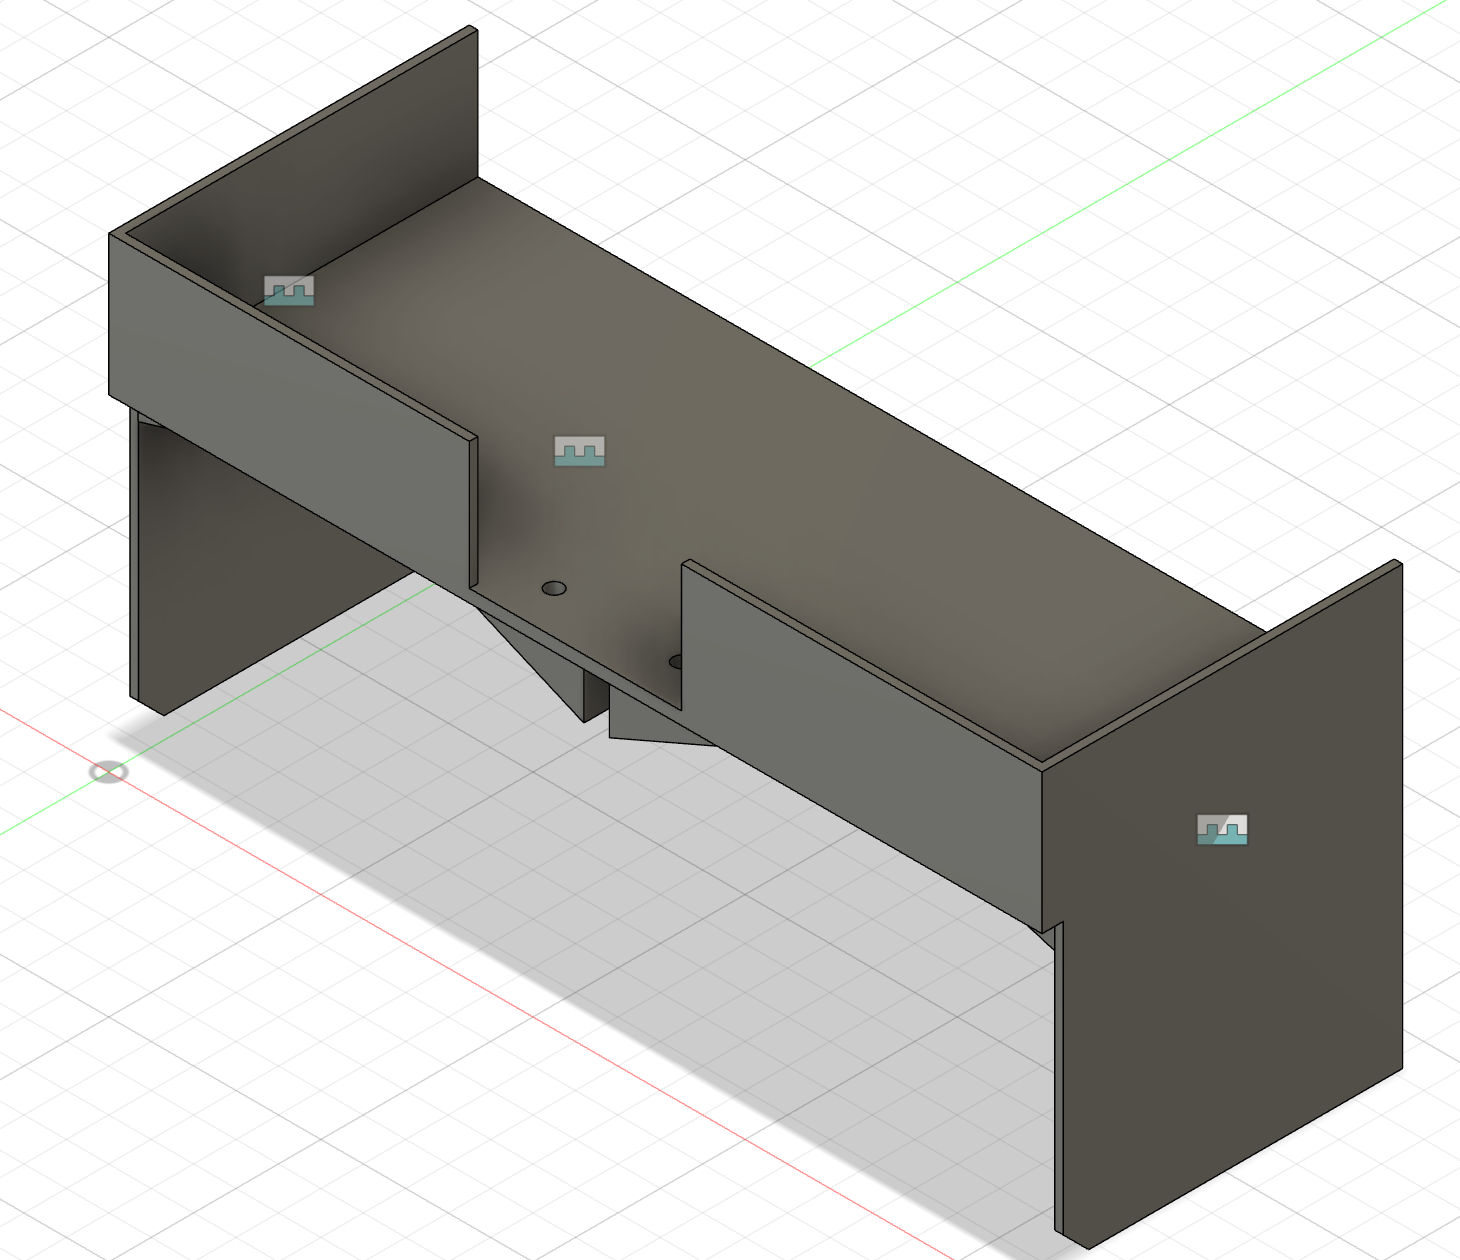
\includegraphics[width=0.7\textwidth]{./graf/upper.png}
%   \caption{Model górnej części obudowy}
%   \label{fig:ball-close}
% \end{figure}

% \begin{figure}[h!]
%   \centering
%   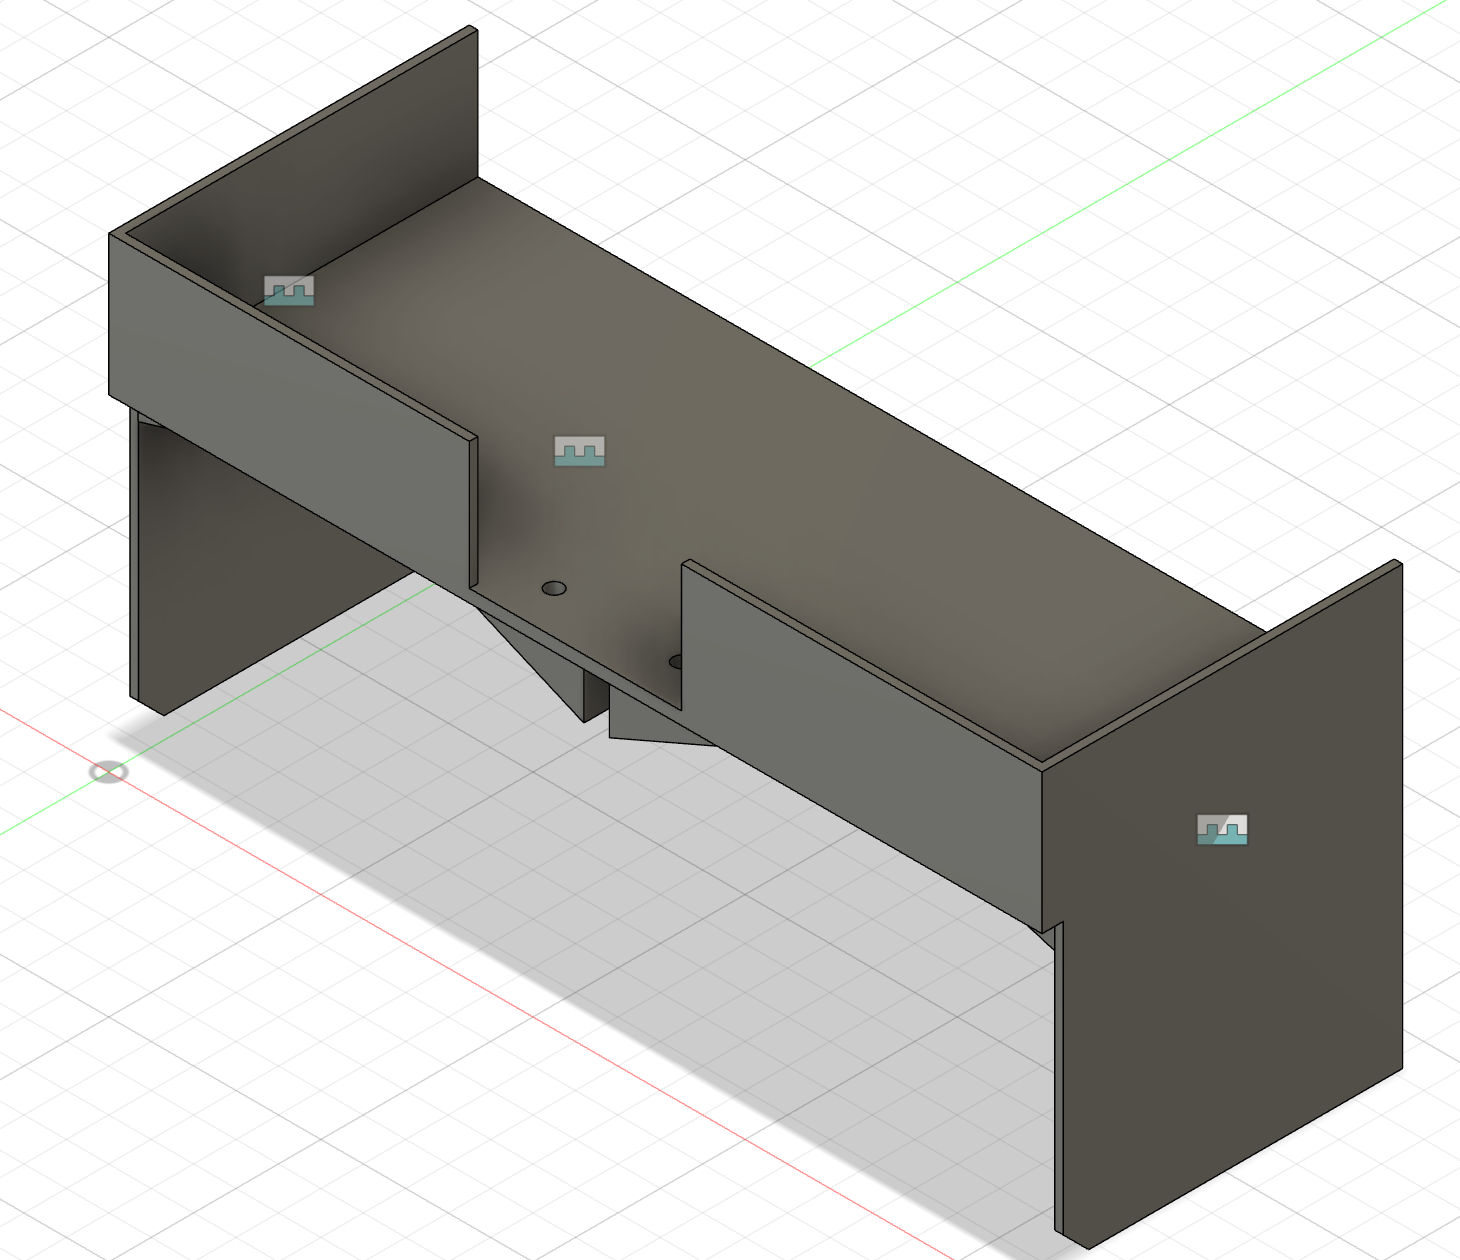
\includegraphics[width=0.7\textwidth]{./graf/upper.png}
%   \caption{Model górnej części obudowy}
%   \label{fig:ball-close}
% \end{figure}

\subsection{Właściwy projekt robota mobilnego}

Po pozytywnym zakończeniu walidacji funkcjonowania algorytmów sterowania i komunikacji, przystąpiono do drugiego etapu konstrukcji – zaprojektowania i wytworzenia docelowej obudowy bazowej robota. Obudowa została wykonana przy użyciu technologii druku 3D, co pozwoliło na uzyskanie wysokiej precyzji oraz wprowadzeniu niezbędnych modyfikacji konstrukcyjnych w stosunku do prototypu. Ze względu na ograniczenia przestrzeni roboczej urządzenia drukującego, wymiary podstawy platformy zostały przeniesione na plan kwadratu o boku 220 mm.
Przednia ściana została zaprojektowana jako część podłogi, w celu zwiększenia sztywności konstrukcji. Najcięższym elementem całego robota jest chwytak wraz z serwomechanizmem, przez co wytrzymałość przedniej ściany oraz podłogi była kluczowa. Zgodnie z osią do wewnątrz robota została poprowadzona przegroda, pełniąca funkcję podpory dla górnej części platformy.
Finalny projekt podstawy, przygotowany w programie Autodesk Fusion 360, został przedstawiony na rysunku [\ref{fig:full}].

\hspace{1cm} 

Ostatni etap obejmował zaprojektowanie górnej części obudowy, na której zostanie osadzony komputer Raspberry Pi oraz przymocowany uchwyt na kamerę. Sposób osadzenia górnej części na dolnym segmencie opiera się na precyzyjnie wykonanej przerwie, w którą wsuwa się wspornik bazy. Dzięki takiemu rozwiązaniu, w prosty i szybki sposób można zdjąć górną część i dokonać potrzebnych zmian lub modyfikacji. Te atrybuty są szczególnie przydatne podczas fazy testów i ciągłego ulepszania robota.

W wersji docelowej, przeznaczonej do komercyjnego użytkowania, omawiane mocowanie zostałoby zastąpione przez standardowe połączenia śrubowe lub sklejenie, co zwiększyłoby trwałość obudowy.

\hspace{1cm}

Ostateczna wersja platformy mobilnej została zaprezentowana na zdjęciu [\ref{fig:base-full}] oraz jest widoczna na nagraniach załączonych do pracy. Model obudowy stanowi w pełni funkcjonalny, zgodny z założeniami, robot, jednak część mocowań w wersji przeznaczonej do sprzedaży należy zmienić. 

W tym celu zastosowano mocowania, umożliwiające łatwe zdejmowanie i zakładanie górnej części obudowy na podstawę, co znacząco ułatwia konserwację oraz serwisowanie wewnętrznych komponentów.

Finalna wersja platformy mobilnej została zaprezentowana na ilustracji \ref{fig:full}, a także na załączonych nagraniach.


\begin{figure}[H]
  \centering
  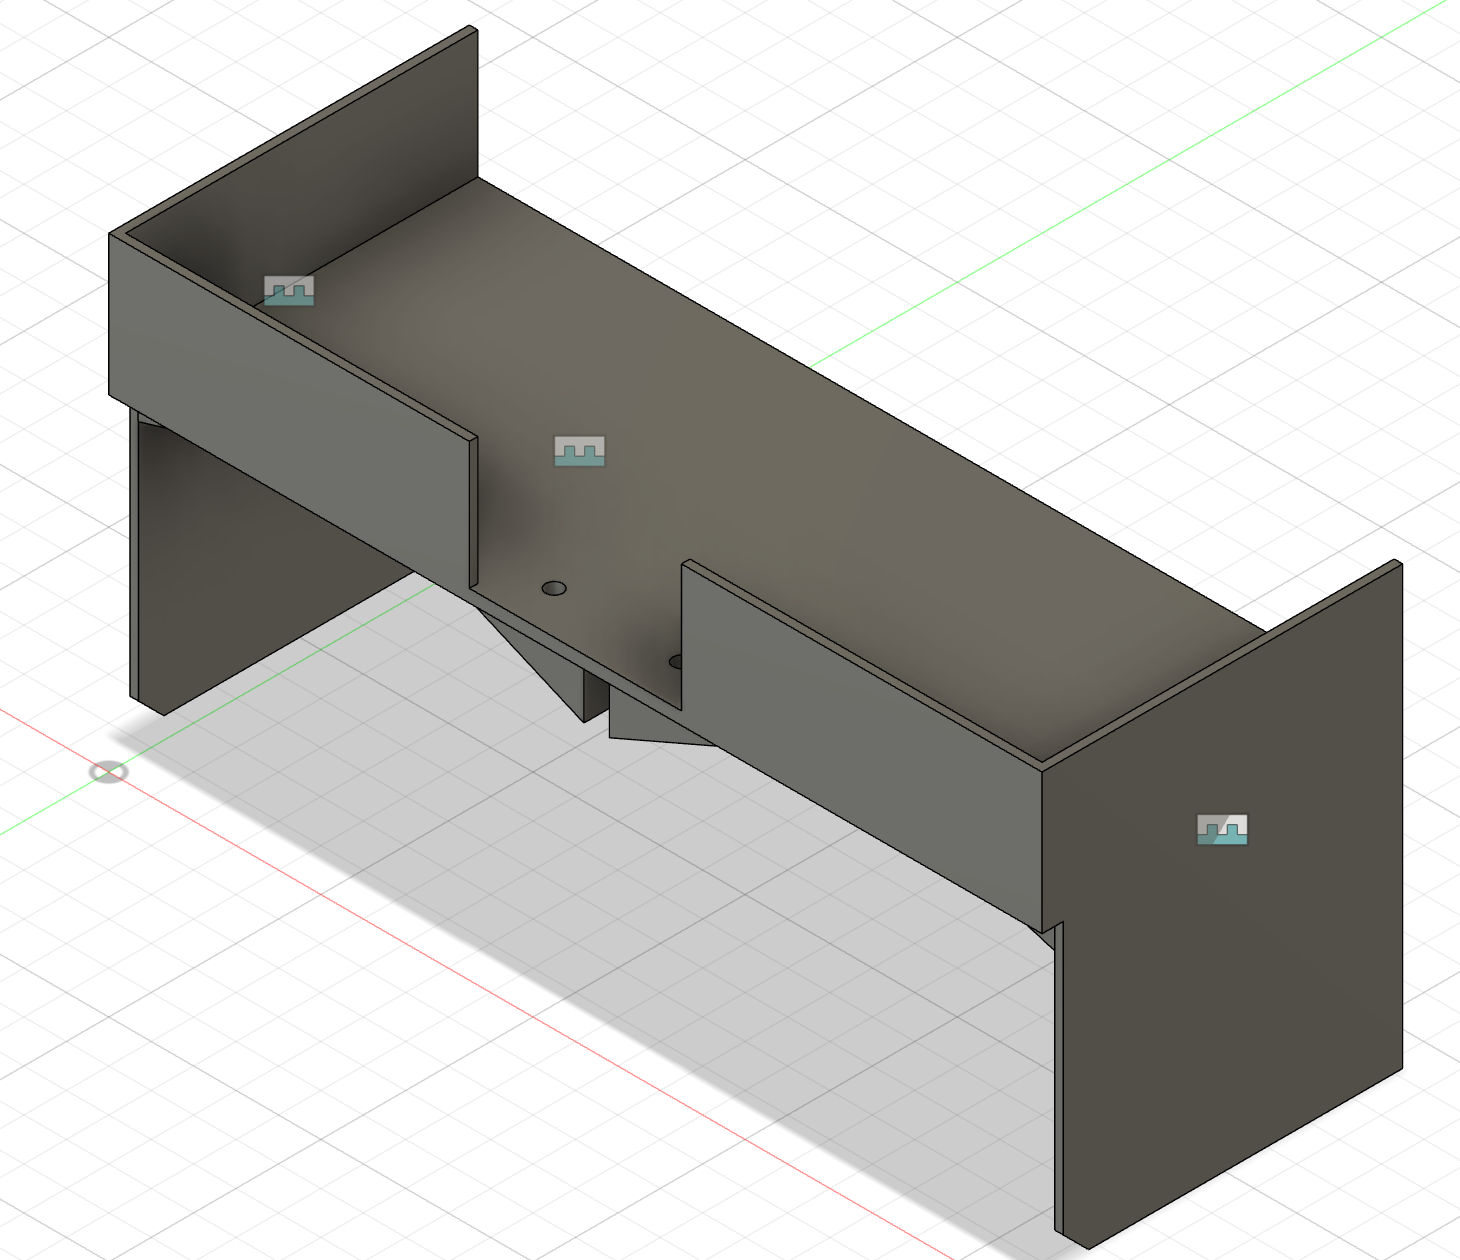
\includegraphics[width=0.7\textwidth]{./graf/upper.png}
  \caption{Model górnej części obudowy}
  \label{fig:ball-close}
\end{figure}

\begin{figure}[H]
  \centering
  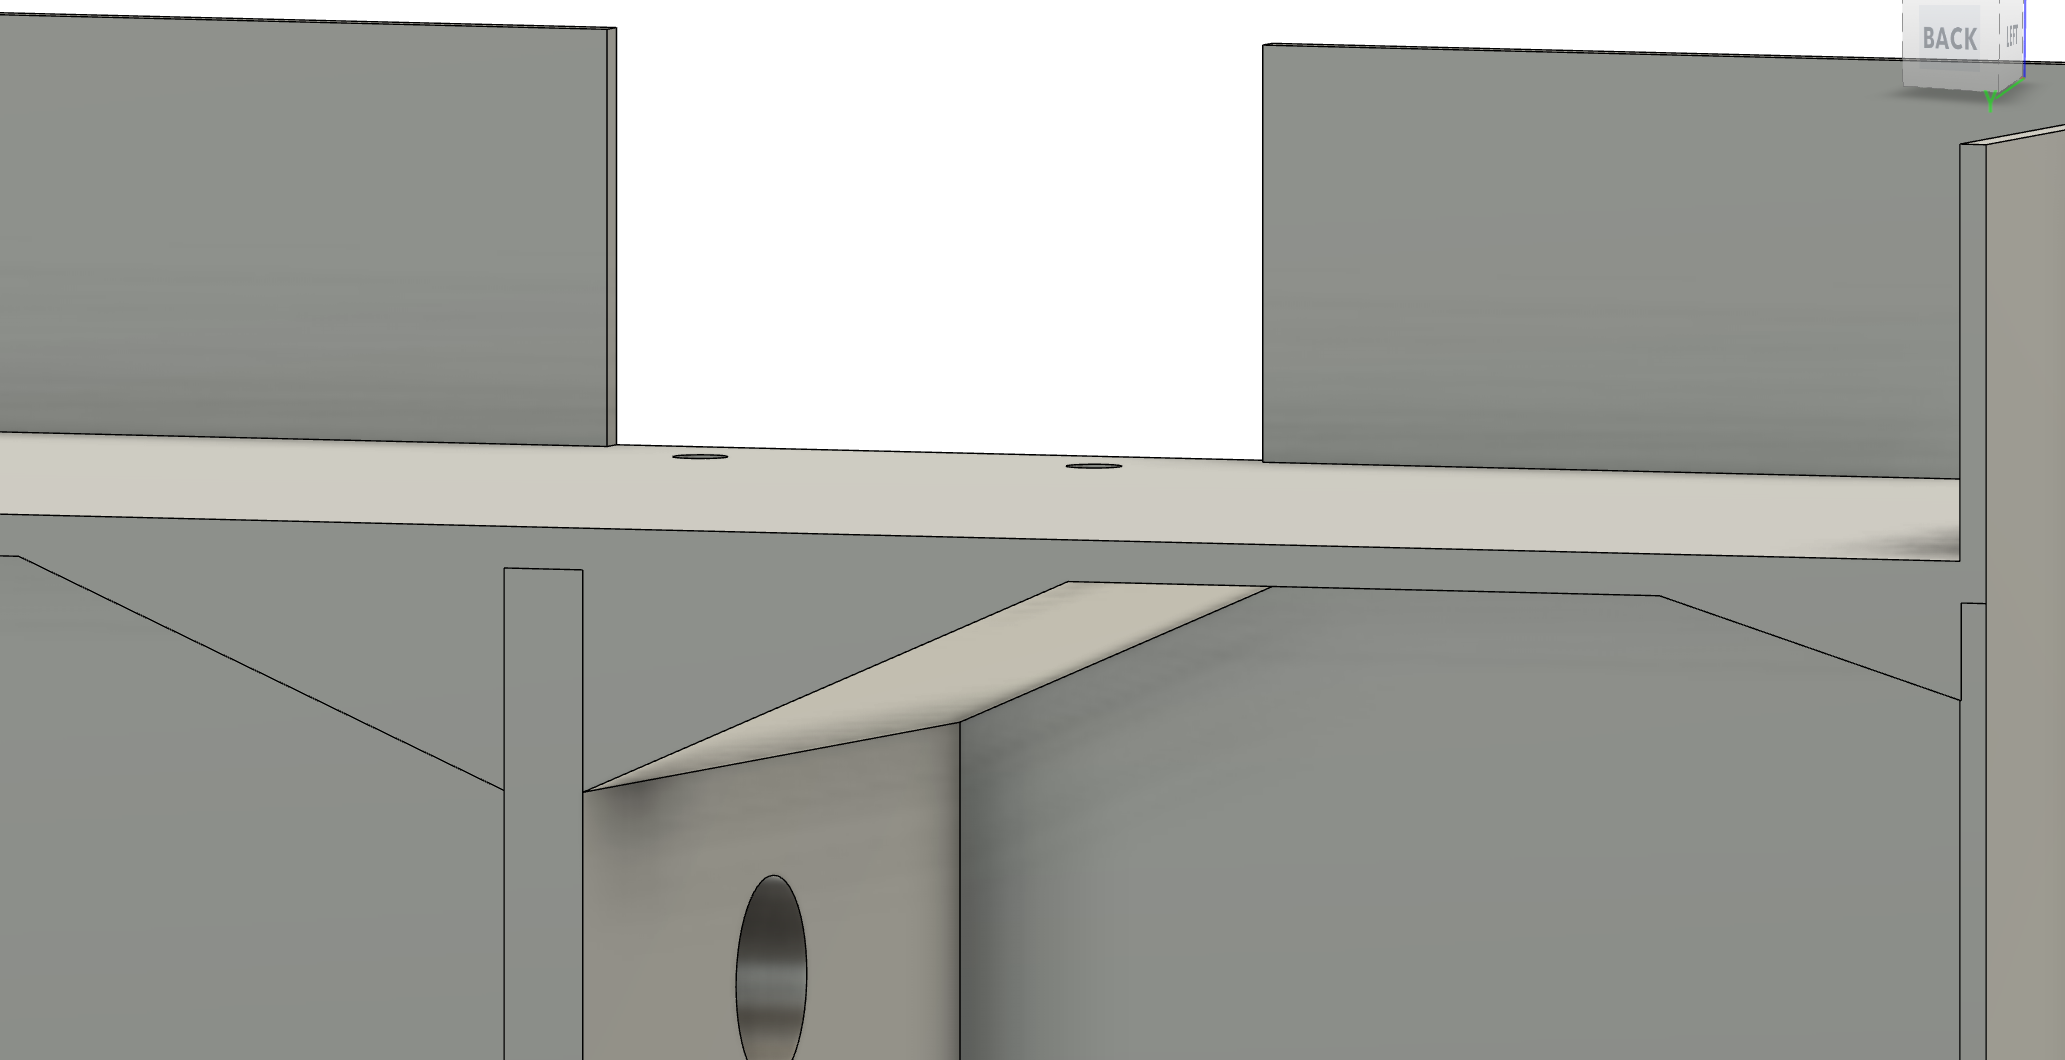
\includegraphics[width=0.7\textwidth]{./graf/full-close.png}
  \caption{Przybliżenie sposobu połączenia górnej części obudowy z dolną. Widoczny jest również otwór przeznaczony na przewody połączeniowe}
  \label{fig:full-close}
\end{figure}


\begin{figure}[H]
  \centering
  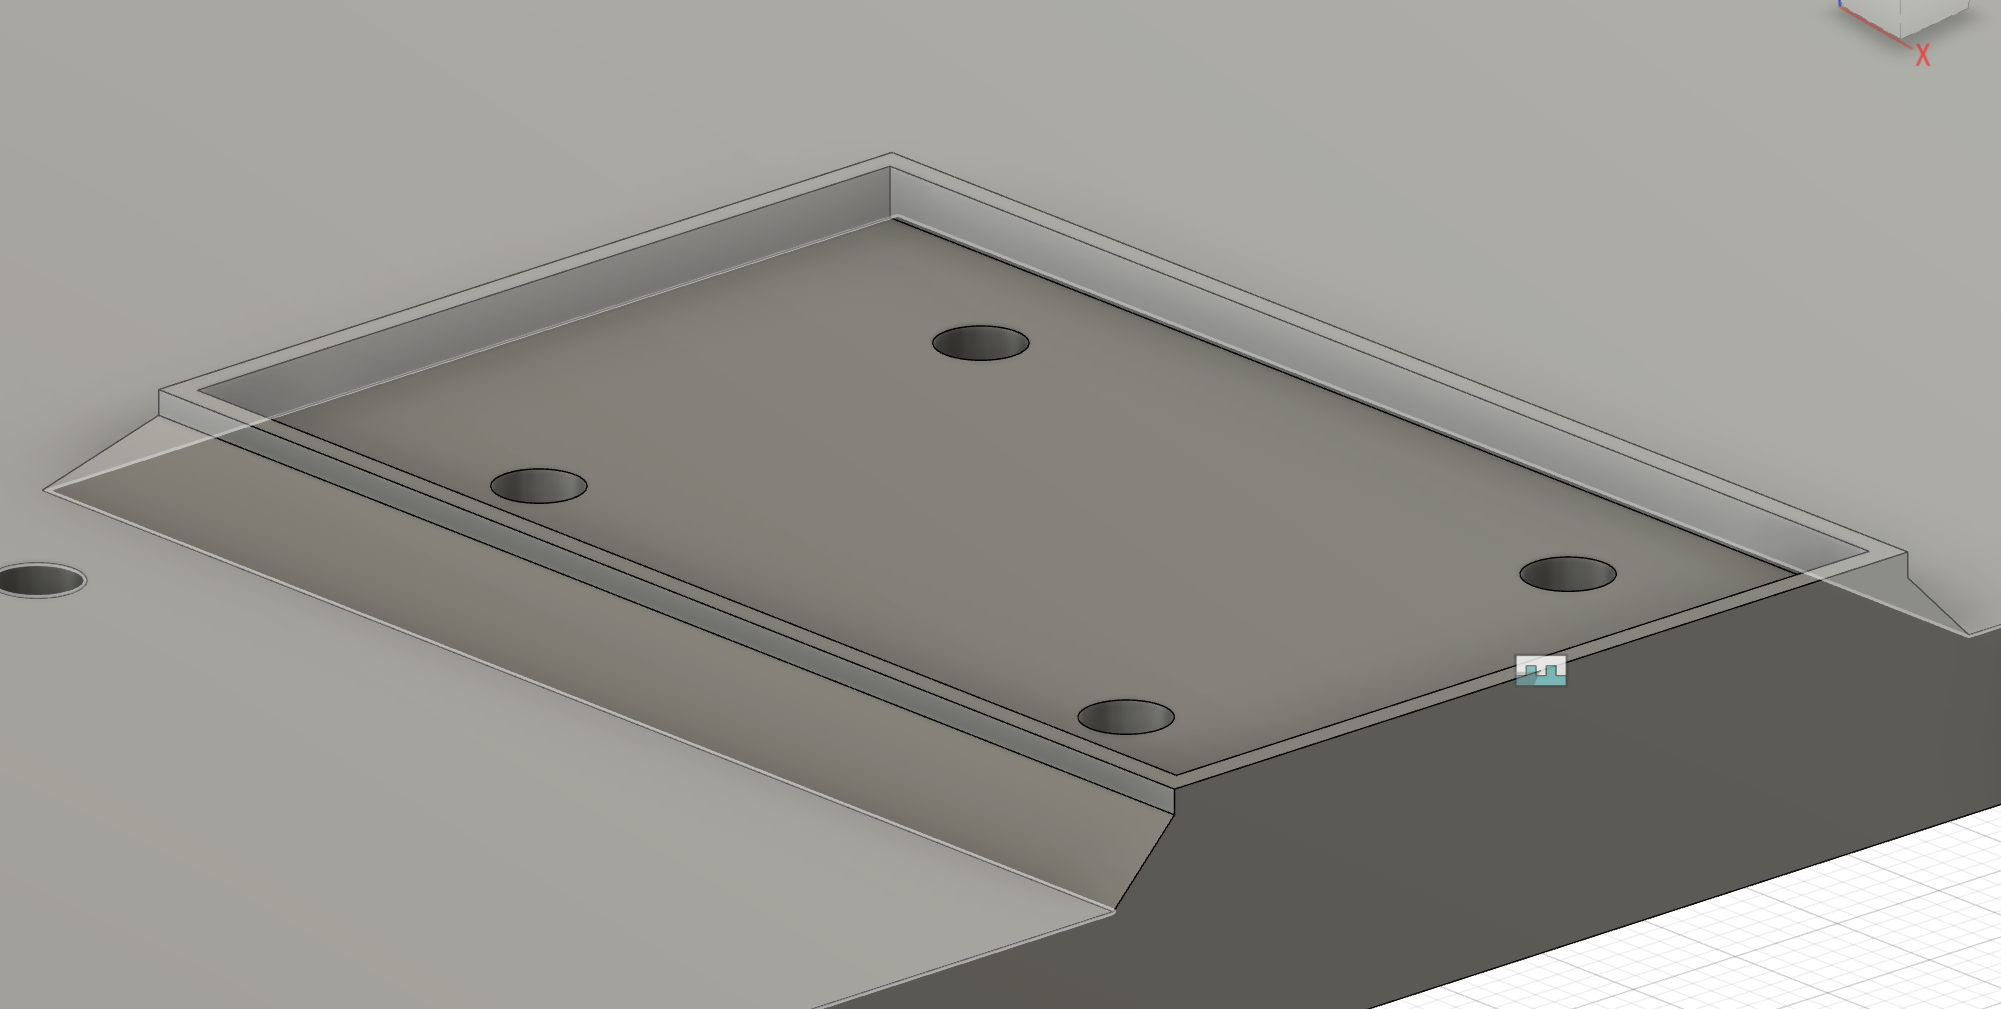
\includegraphics[width=0.5\textwidth]{./graf/motor-close.png}
  \caption{Przybliżenie miejsca na mocowania silników}
  \label{fig:base-close}
\end{figure}

\begin{figure}[H]
  \centering
  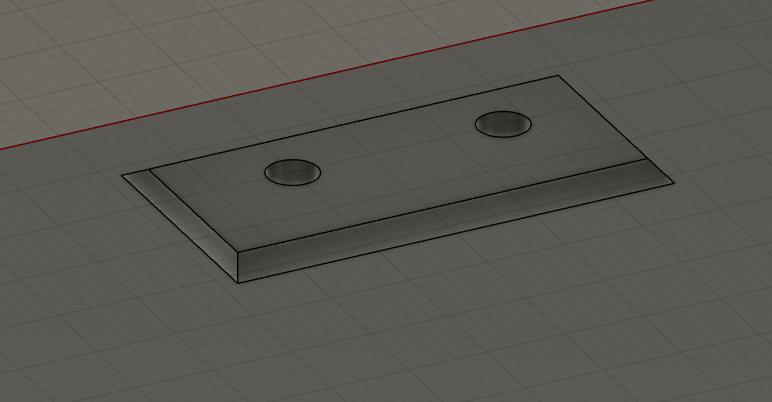
\includegraphics[width=0.5\textwidth]{./graf/ball-close.png}
  \caption{Przybliżenie miejsca mocowania kulek podporowych w osi robota}
  \label{fig:ball-close}
\end{figure}

\begin{figure}[H]
  \centering
  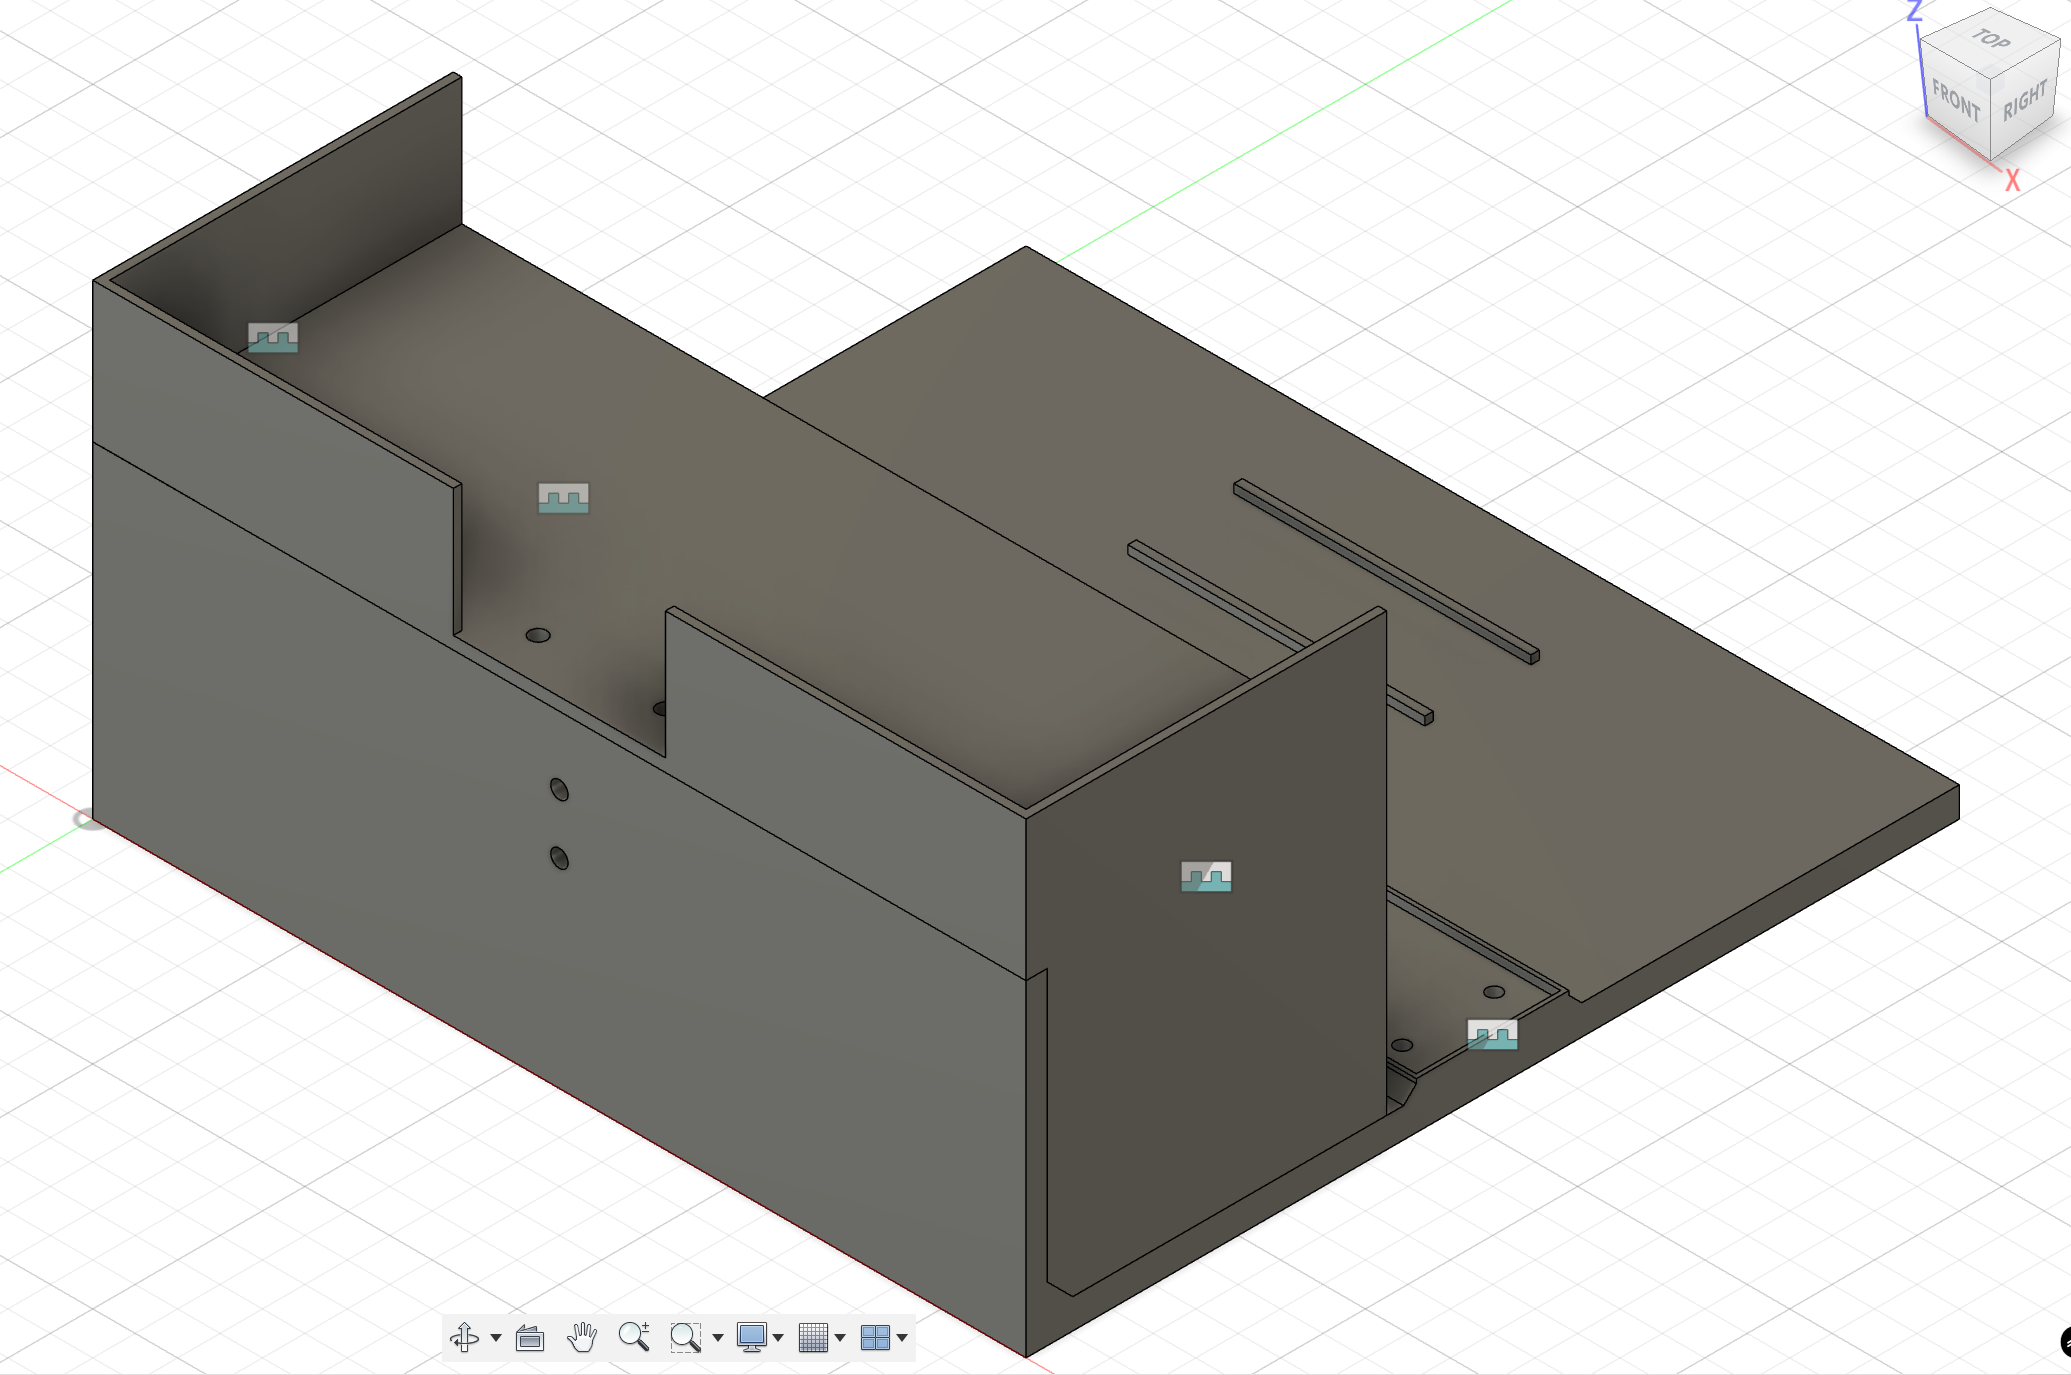
\includegraphics[width=0.9\textwidth]{./graf/full.png}
  \caption{Prezentacja finalnej wersji obudowy robota}
  \label{fig:full}
\end{figure}
 
\clearpage

\section{Implementacja kontrolera silników}

Aplikacja kontrolera silników została zaimplementowana w środowisku Arduino IDE, co było podyktowane użyciem mikrokontrolera ATMega328P na płytce Arduino UNO R3. Zadaniem kontrolera było wysyłanie odpowiednich sygnałów PWM do sterownika silników oraz zliczanie impulsów enkoderów w celu uzyskania pożądanej dokładności. 

W tej sekcji opisano kluczowe elementy aplikacji, w tym konfigurację pinów, algorytmy sterujące oraz komunikację z komputerem Raspberry Pi.

\subsection{Konfiguracja pinów i ustawienia PWM}

W kontrolerze skonfigurowano piny odpowiadające za obsługę enkoderów oraz sterowanie kierunkiem i prędkością silników za pomocą sygnałów PWM. Poniższy kod definiuje przypisanie pinów do odpowiednich funkcji, takich jak odczyt kanałów enkoderów oraz wyjść sterujących silnikami:

\begin{figure}[h!]
  \centering
  \begin{lstlisting}
    // Encoders pins
    #define ENCA1 2 
    #define ENCA2 3 
    
    // Motor driver pins
    #define PWM1 10
    #define DIR1 13
    #define PWM2 11
    #define DIR2 12
    
    // Servo PWM pin
    #define SERVO_PIN 9
  \end{lstlisting}
  \caption{Fragment przedstawiający konfigurację pinów}
  \label{fig:config}
\end{figure}

\subsection{Algorytm sterowania PID}

Algorytm sterowania PID odpowiada za utrzymanie zadanej prędkości kątowej każdego z silników poprzez dostosowanie sygnału PWM. Wyjście regulatora PID jest obliczane na podstawie bieżącego błędu pozycji enkodera, wartości całki i pochodnej błędu. Parametry regulatora, takie jak wzmocnienie proporcjonalne (\texttt{Kp}), całkujące (\texttt{Ki}) oraz różniczkujące (\texttt{Kd}), zostały dobrane empirycznie i wynoszą:

\begin{figure}[h!]
  \centering
  \begin{lstlisting}
    float Kp = 1.0; 
    float Ki = 0.5; 
    float Kd = 0.1; 
  \end{lstlisting}
  \caption{Wartości parametrów regulatora PID}
  \label{fig:config-pid}
  \end{figure}

Na podstawie obliczonego błędu funkcja \texttt{performDrive()} dokonuje aktualizacji sygnału sterującego dla każdego silnika, uwzględniając przy tym warunki zatrzymania po osiągnięciu zadanej pozycji. Wartość wyjścia jest ograniczana do przedziału \( \pm 70 \), aby zapobiec zbyt dużemu skokowi napięcia sterującego:

\begin{figure}[h!]
  \centering
  \begin{lstlisting}
    float error1 = targetCountsWheelRight - abs(pos1);
    float error2 = targetCountsWheelLeft - abs(pos2);
    float output1 = 0;
    float output2 = 0;
    unsigned long currT = micros();
    float deltaT = (currT - prevT) / 1e6;
    prevT = currT;

    if(!stopCond1){
      integral1 = error1 * deltaT;
      float derivative1 = (error1 - previousError1) / deltaT;
      output1 = Kp * error1 + Ki * integral1 + Kd * derivative1;

      output1 = constrain(output1, -55, 55);
      if (output1 > 0 && output1 < 30) output1 = 30;
      if (output1 < 0 && output1 > -30) output1 = -30;

      if (abs(error1) > tolerance && targetCounts != 0) {
          setMotor(1, abs(output1), PWM1, DIR1);
      } else {
          stopCond1 = true;
          setMotor(1, 0, PWM1, DIR1);
      }
    }
  \end{lstlisting}
  \caption{Fragment przedstawiający realizację regulacji PID}
  \label{fig:pseudokod:pid}
\end{figure}

Dodatkowo został wykorzystany globalny marker \textit{stopCond1} odpowiedzialny za podtrzymanie silnika pierwszego (lub adekwatnie drugiego) w sytuacji, gdy pierwszy z nich zakończy pracę. Ze względu na pewną bezwładność silnika i dużą czułość enkoderów, brak zastosowania tej zmiennej skutkował nieskończonym działaniem pętli. 

\subsection{Funkcja zliczająca impulsy enkoderów}

Dla uzyskania dokładnych odczytów pozycji, w kontrolerze zastosowano obsługę przerwań na pinach podłączonych do enkoderów. Funkcje \texttt{readEncoder1()} i \texttt{readEncoder2()} zliczają impulsy z enkoderów, aktualizując wartość liczników pozycji. W ten sposób każda zmiana sygnału na kanale enkodera jest przetwarzana w czasie rzeczywistym, co umożliwia precyzyjne śledzenie pozycji kół:

\begin{figure}[h!]
  \centering
  \begin{lstlisting}   
  void readEncoder1() {
    int MSB1 = digitalRead(ENCA1);

    if (MSB1) {  
      posi1++;  
    }
  }

  void readEncoder2() {
    int MSB2 = digitalRead(ENCA2);

    if (MSB2) {  
      posi2++; 
    }
  }
  \end{lstlisting}
  \caption{Funkcja zliczająca impulsy enkodera}
  \label{fig:enc-count}
\end{figure}

\subsection{Realizacja komunikacji z Raspberry Pi}

Komunikacja została zaimplementowana z wykorzystaniem ramki bitowej składającej się z dwóch bajtów. Pierwszy bajt odpowiada za przekazanie informacji o typie ruchu takich jak:
\begin{itemize}
  \item Typ ruchu - czy jest to ruch do przodu czy skręt.
  \item Kierunek ruchu - jeśli typ ruchu to skręt, ten bit odkreśla kierunek, w który robot ma się przemieścić.
  \item Ruch serwa - flaga określająca czy serwo ma wykonać ruch.
  \item Typ ruchu serwa - informuje mikrokontroler, czy serwo powinno się zamknąć czy otworzyć. 
\end{itemize}

Drugi bajt odpowiada za przekazanie informacji o odległości jaką ma przejechać robot lub o jaki kąt powinien się obrócić. 

Odczyt z magistrali szeregowej odbywa się w momencie, gdy są możliwe do odczytania dokładnie dwa bajty. Zrealizowane jest to za pomocą wbudowanej funkcji \textit{Serial.available() >= 2}. Jeżeli warunek jest spełniony następuje odczytanie zawartości ramki oraz przepisanie jej wartości do zmiennych globalnych mikrokontrolera. 

Fragment kodu realizujący odczyt znajduje się poniżej.

\begin{figure}[h!]
  \centering
  \begin{lstlisting}
    if (Serial.available() >= 2) {  
      
      firstByte = Serial.read();
      secondByte = Serial.read();

      movementType = (firstByte & 0b11000000) >> 6;

      dir = (firstByte & 0b00100000) >> 5;

      servo = (firstByte & 0b00010000) >> 4;

      servoAction = (firstByte & 0b00001000) >> 3;

      stopCond1 = false;
      stopCond2 = false;
  \end{lstlisting}
  \caption{Fragment przedstawiający odczyt ramki bitowej z magistrali szeregowej}
  \label{fig:read-uart}
\end{figure}

\subsection{Pętla główna programu}

Pętla główna programu opiera się na sprawdzaniu warunku dostępności dwóch bajtów w magistrali szeregowej. Jeżeli nie ma żadnych danych lub jest ich za mało, program przechodzi do sprawdzania kolejnych warunków. Jeżeli nastąpił odczyt, któryś z ich na pewno zostanie spełniony. 

W kolejnych instrukcjach warunkowych znajdują się wywołania odpowiednich funkcji, realizujących ruch. Każda funkcja wykonawcza zwraca wartość typu \textit{Boolean}, a więc prawda lub fałsz. Jeżeli zadanie zostanie poprawnie zrealizowane, zwrócona zostanie wartość \english{true}, a tym samym ostatnia instrukcja warunkowa, wysyłająca informację do komputera Raspberry Pi informację, że zadanie zostało ukończone i można przejść do kolejnej instrukcji oraz następuje wyzerowanie zmiennych. 

Fragment realizujący zarządzanie zadaniami znajduje się poniżej. 

\begin{figure}[h!]
  \centering
  \begin{lstlisting}
    if(movementType == 1 && targetCounts != 0){
      if(dir == 1){
        status = performTurn(1, -1);
      } else {
        status = performTurn(-1, 1);
      }
      // status = dir == 1 ? performTurn(1, -1) : performTurn(-1, 1);
    }
    else if(movementType == 0 && targetCounts != 0){
      status = performDrive();
    }
    
    if(servo){
      //Serial.print("Servo Func evoke: ");
      status = performGrab(servoAction);
    }
  
    if (status) {
      sprintf(res, "FINISH -> P1: %d | P2: %d | E1: %d | E2: %d", P1, P2, E1, E2);
      Serial.println(res);
      targetCounts=0;
      targetCountsWheelRight = 0;
      targetCountsWheelLeft = 0;
      status = false;
    }
  \end{lstlisting}
  \caption{Fragment przedstawiający logikę zarządzania otrzymanym zadaniem}
  \label{fig:manage-ex}
\end{figure}

\clearpage

\section{Implementacja głównej aplikacji sterującej}

Główna aplikacja sterująca, odpowiedzialna za zarządzanie operacjami robota, została napisana w języku Python w wersji 3.10. W aplikacji tej wykorzystano biblioteki takie jak OpenCV (do przetwarzania obrazu), \textit{pyserial} (do komunikacji szeregowej z mikrokontrolerem) oraz \textit{threading} (do zarządzania współbieżnością zadań). Aplikacja działa w trybie konsolowym, co pozwala na jej zdalne uruchomienie i kontrolowanie za pomocą protokołu SSH.


\subsection{Opis funkcji głównej aplikacji \texttt{mainTask()}}

Funkcja \texttt{mainTask()} pełni rolę głównej pętli zarządzającej działaniem aplikacji. Po uruchomieniu prezentuje użytkownikowi menu opcji sterujących, umożliwiających wybór trybu pracy robota: trybu automatycznego, trybu manualnego, otwarcia panelu operatorskiego lub zakończenia działania aplikacji. Umożliwia także płynne zarządzanie procesami robota przy użyciu współbieżnych podprocesów uruchamianych za pomocą biblioteki \texttt{threading}.

W poniższym kodzie, fragment wstępny inicjalizuje odpowiednie elementy biblioteki \texttt{threading}, takie jak flaga statusu \texttt{status} (typ \texttt{Event}), która umożliwia asynchroniczne monitorowanie stanu zakończenia poszczególnych zadań, co pozwala na bezpieczne zakończenie każdego procesu:

\begin{figure}[h!]
  \centering
  \begin{lstlisting}
import threading
import time
import os
import sys

# Configuration of module path
module_path = os.path.abspath('/home/jakub/engineering_proj/robot-control-system/current_v2')
sys.path.insert(0, module_path)

# Importing modules
from serial_communication import SerialCommunication
from auto_control_mode import AutoModeModule
from camera_module import CameraModule
from web_app.app import WebAppVisu
  \end{lstlisting}
  \caption{Importowanie bibliotek i modułów sterujących aplikacją}
  \label{fig:imported_modules}
\end{figure}

W kolejnych sekcjach opisano szczegółowo działanie każdej z dostępnych opcji w funkcji \texttt{mainTask()}.

\subsubsection{Tryb automatyczny}

Tryb automatyczny, aktywowany wyborem opcji 1, uruchamia niezależny wątek kontrolujący działanie robota w sposób autonomiczny. Wątek ten realizuje operacje poprzez funkcję \texttt{start\_auto\_control\_task()}, której zadaniem jest uruchomienie instancji klasy \texttt{AutoModeModule}. Klasa ta, poprzez wywołanie metody \texttt{selectPath()}, realizuje sekwencję ruchów oraz operacji robota w trybie w pełni autonomicznym, umożliwiając monitorowanie postępu poprzez zmienną \texttt{status}.

Wątek \texttt{auto\_control\_thread} jest uruchamiany wewnątrz instrukcji \texttt{try-except}, co zabezpiecza program przed niespodziewanymi wyjątkami w trakcie jego działania, jak pokazano poniżej:

\begin{figure}[h!]
  \centering
  \begin{lstlisting}
if choice == '1':
    try:
        auto_control_thread = threading.Thread(target=start_auto_control_task, args=(serial_com, status))
        auto_control_thread.start()
        print("Auto mode has started")

        # Monitoring the auto mode until finished
        while not status.is_set():
            time.sleep(0.01)
        auto_control_thread.join()
        print("Auto mode has finished")
    except:
        print("Exception occurred during attempt to perform auto control")
  \end{lstlisting}
  \caption{Wybór i uruchomienie trybu automatycznego}
  \label{fig:automode_choice}
\end{figure}

Funkcja \texttt{start\_auto\_control\_task()} wykorzystuje klasę \texttt{AutoModeModule} do komunikacji z mikrokontrolerem przez port szeregowy oraz wywołuje zadania w pętli głównej.

\subsubsection{Tryb ręczny i panel operatorski}

Opcja 2, reprezentująca tryb manualny, jest zarezerwowana na dalszą implementację, umożliwiając użytkownikowi kontrolę robota w czasie rzeczywistym za pomocą klawiatury.

Opcja 3 natomiast uruchamia wątek \texttt{camera\_module\_task}, który włącza panel operatorski z wizualizacją kamery przy użyciu biblioteki OpenCV. Działa on poprzez funkcję \texttt{start\_web\_app\_task()}, która inicjalizuje obiekt klasy \texttt{WebAppVisu} i wywołuje metodę \texttt{run()} odpowiedzialną za uruchomienie serwera aplikacji wizualizacyjnej. Wybór trybu ręcznego i uruchomienie panelu operatorskiego przedstawiono poniżej:

\begin{figure}[h!]
  \centering
  \begin{lstlisting}
elif choice == '3':
    try:
        camera_module_task = threading.Thread(target=start_web_app_task)
        camera_module_task.start()
        print("Camera task has started correctly")
    except:
        print("Exception occurred during attempt to start camera Task")
  \end{lstlisting}
  \caption{Uruchomienie panelu operatorskiego z wizualizacją}
  \label{fig:panel_task}
\end{figure}

\subsubsection{Zakończenie działania aplikacji}

Wybór opcji 5 inicjuje procedurę zakończenia pracy programu. Zaimplementowana instrukcja warunkowa sprawdza, czy wątek \texttt{auto\_control\_thread} jest aktywny. W przypadku jego działania ustawiany jest \texttt{status} jako zakończony, co umożliwia bezpieczne zamknięcie wątku poprzez wywołanie metody \texttt{join()}, a następnie bezpieczne zamknięcie aplikacji.

\begin{figure}[h!]
  \centering
  \begin{lstlisting}
elif choice == '5':
    if auto_control_thread and auto_control_thread.is_alive():
        status.set()
        auto_control_thread.join()
        print("Exiting ... ")
    break
  \end{lstlisting}
  \caption{Kod zamykający wątki i kończący działanie aplikacji}
  \label{fig:app_exit}
\end{figure}

\subsubsection{Inicjalizacja funkcji pomocniczych}
 
Funkcja \texttt{start\_auto\_control\_task()} inicjuje działanie klasy \texttt{AutoModeModule}, która umożliwia pełną kontrolę autonomicznego poruszania się robota oraz wybór i realizację zadań. Obiekt tej klasy, przekazany przez parametr, komunikuje się z mikrokontrolerem, przesyłając komendy dotyczące prędkości i kierunku poruszania się.

Dodatkowo, funkcja \texttt{start\_web\_app\_task()} inicjuje aplikację wizualizacyjną \texttt{WebAppVisu}, umożliwiającą przesyłanie i odbiór danych z kamery robota, co daje operatorowi podgląd w czasie rzeczywistym.

\begin{figure}[h!]
  \centering
  \begin{lstlisting}
def start_auto_control_task(serial_com, status):
    auto_module = AutoModeModule(serial_com, status)
    auto_module.selectPath()

def start_web_app_task():
    web_app = WebAppVisu()
    web_app.run()
  \end{lstlisting}
  \caption{Kod funkcji uruchamiających zadania kontrolne robota}
  \label{fig:tasks_start}
\end{figure}

\subsection{Opis sposobu komunikacji szeregowej}

Komunikacja szeregowa między jednostką sterującą (Raspberry Pi) a mikrokontrolerem (Arduino) jest realizowana za pomocą dedykowanej klasy \texttt{SerialCommunication}. Klasa ta została zaprojektowana w celu zapewnienia niezawodnej i bezpiecznej wymiany danych poprzez interfejs szeregowy z wykorzystaniem formatu binarnego, co umożliwia precyzyjne przekazywanie instrukcji do mikrokontrolera.

\subsubsection{Inicjalizacja połączenia szeregowego}

Klasa \texttt{SerialCommunication} otwiera połączenie szeregowe na wybranym porcie (w tym przypadku \texttt{/dev/ttyUSB0}) oraz ustawia szybkość transmisji (baud rate) na poziomie 250000 bps, co pozwala na szybkie przesyłanie danych w czasie rzeczywistym. Podczas inicjalizacji sprawdzane jest, czy port został otwarty poprawnie, a następnie następuje reset buforów wejściowego i wyjściowego w celu zapewnienia spójności przesyłanych danych.

\begin{figure}[h!]
  \centering
  \begin{lstlisting}
def __init__(self):
    self.ser = serial.Serial('/dev/ttyUSB0', 250000, timeout=1)

    if self.ser.is_open:
        print("Serial port is open")

    self.ser.reset_input_buffer()
    self.ser.reset_output_buffer()
  \end{lstlisting}
  \caption{Kod inicjalizujący połączenie szeregowe}
  \label{fig:serial_init}
\end{figure}

\subsubsection{Wysyłanie danych do Arduino}

Metoda \texttt{send\_data} w klasie \texttt{SerialCommunication} odpowiada za przesyłanie preformatowanych instrukcji (dwubajtowych ramek binarnych) do Arduino. Funkcja przyjmuje jako argument \texttt{bytearray}, który reprezentuje ramkę danych składającą się z informacji dotyczących typu oraz parametrów ruchu robota. Każda ramka binarna jest zapisywana bezpośrednio do portu szeregowego jako surowe dane binarne, co zapewnia, że dane przesyłane są dokładnie w formacie oczekiwanym przez Arduino, bez dodatkowych konwersji.

\begin{figure}[h!]
  \centering
  \begin{lstlisting}
def send_data(self, data):
    try:
        # Wyślij ramkę danych
        self.ser.write(data)  
        print(f"The binary message {data} has been sent")
        time.sleep(4) 
  \end{lstlisting}
  \caption{Kod odpowiedzialny za wysyłanie danych do Arduino}
  \label{fig:serial_send}
\end{figure}

\subsubsection{Odbiór i potwierdzenie zakończenia operacji}

Po wysłaniu ramki \texttt{send\_data} oczekuje na potwierdzenie zakończenia zadania przez Arduino, które przesyła odpowiedź tekstową zawierającą frazę \texttt{"FINISH"} po zakończeniu zadanej operacji ruchu. Oczekiwanie na odpowiedź realizowane jest poprzez sprawdzenie, czy w buforze wejściowym pojawiły się dane do odczytu.

W przypadku obecności danych w buforze, metoda odczytuje zawartość jako strumień bajtów, konwertuje na tekst i sprawdza, czy zawiera on potwierdzenie zakończenia. Jeśli Arduino przesłało frazę \texttt{"FINISH"}, metoda zwraca wartość \texttt{True}, co wskazuje, że zadanie zostało wykonane pomyślnie. W przeciwnym razie, jeśli brak jest danych w buforze lub wystąpił błąd, metoda zwraca \texttt{False}.

\begin{figure}[h!]
  \centering
  \begin{lstlisting}
# Sprawdź, czy są dostępne dane do odczytu
if self.ser.in_waiting > 0:
    dane = b"" 

    while self.ser.in_waiting > 0:
        dane += self.ser.read(self.ser.in_waiting)
        
    dane_str = dane.decode('utf-8', errors='ignore')
    print("Received data: ", dane_str)  

    if "FINISH" in dane_str:
        print('Arduino confirmed movement completion.')
        return True
else:   
    print("No incoming data!")
    return False
  \end{lstlisting}
  \caption{Kod odbierający dane potwierdzające zakończenie zadania}
  \label{fig:serial_receive}
\end{figure}

\subsubsection{Obsługa błędów w komunikacji szeregowej}

Komunikacja szeregowa między Raspberry Pi a Arduino, mimo że jest stosunkowo niezawodna, może być podatna na błędy związane z zakłóceniami lub nieoczekiwanym przerwaniem połączenia. W związku z tym metoda \texttt{send\_data} zabezpieczona jest instrukcją \texttt{try-except}, która wyłapuje wyjątki występujące podczas przesyłania danych. W przypadku wykrycia błędu zostaje wyświetlony komunikat o błędzie, a metoda zwraca \texttt{False}, co sygnalizuje niepowodzenie wykonania zadania.

Dzięki temu rozwiązaniu aplikacja jest bardziej odporna na nieprzewidziane błędy i może odpowiednio reagować w sytuacjach awaryjnych, takich jak utrata łączności.

\begin{figure}[h!]
  \centering
  \begin{lstlisting}
    except Exception as e:
      print(f'Exception occurred during serial communication: {e}')
      return False
  \end{lstlisting}
  \caption{Obsługa błędów komunikacji szeregowej}
  \label{fig:serial_exception}
\end{figure}

\subsection{Opis sposobu detekcji klocka oraz rozpoznawania koloru}

Moduł kamery odpowiedzialny jest za detekcję klocków oraz rozpoznawanie ich kolorów w obrazie wideo na podstawie analizy kolorów w przestrzeni barw HSV oraz konturów. Realizacja tego zadania opiera się na przetwarzaniu strumienia wideo, który jest przechwytywany za pomocą kamery, a następnie przekształcany w czasie rzeczywistym. Klasa \texttt{CameraModule} zarządza procesem przechwytywania i analizowania obrazu, natomiast funkcje pomocnicze realizują zadania związane z maskowaniem kolorów, identyfikacją konturów oraz rozpoznawaniem charakterystycznych kształtów, takich jak kwadrat.

\subsubsection{Definicja zakresów kolorów}

Aby zidentyfikować kolory klocków, każdy kolor definiowany jest przez odpowiedni zakres wartości HSV. Zakresy te określają dolną i górną granicę składowych H (Hue), S (Saturation) i V (Value), umożliwiając tworzenie masek kolorystycznych, które izolują wybrane kolory w obrazie.

\begin{figure}[h!]
  \centering
  \begin{lstlisting}
colors = {
    'blue': [np.array([95, 255, 85]), np.array([120, 255, 255])],
    'red': [np.array([161, 165, 127]), np.array([178, 255, 255])],
    'yellow': [np.array([16, 0, 99]), np.array([39, 255, 255])],
    'green': [np.array([33, 19, 105]), np.array([77, 255, 255])],
    'white': [np.array([0, 0, 200]), np.array([180, 50, 255])],
}
  \end{lstlisting}
  \caption{Definicje zakresów kolorów dla identyfikacji klocków}
  \label{fig:color_definitions}
\end{figure}

\subsubsection{Detekcja koloru}

Funkcja \texttt{find\_color} przetwarza obraz w przestrzeni HSV w celu detekcji zadanych kolorów. Tworzy maskę kolorystyczną przy użyciu wcześniej zdefiniowanych zakresów HSV, a następnie identyfikuje kontury zgodne z kolorem poszukiwanego klocka. W procesie tym uwzględniane są jedynie kontury o powierzchni większej niż ustalony próg (5000 pikseli), co pozwala eliminować drobne zakłócenia.

Dla każdego wykrytego konturu obliczane są jego momenty, co umożliwia wyznaczenie środka masy (współrzędnych \texttt{cx} oraz \texttt{cy}). Jeśli kolorowy kontur zostanie wykryty, funkcja zwraca kontur oraz jego położenie, co pozwala na dalsze przetwarzanie w klasie \texttt{CameraModule}.

\begin{figure}[h!]
  \centering
  \begin{lstlisting}
def find_color(frame, points):
    mask = cv2.inRange(frame, points[0], points[1])  # Create mask with boundaries
    cnts = cv2.findContours(mask, cv2.RETR_TREE, cv2.CHAIN_APPROX_SIMPLE)
    cnts = imutils.grab_contours(cnts)

    for c in cnts:
        area = cv2.contourArea(c)  # Calculate the area of the contour
        if area > 5000:
            M = cv2.moments(c)
            if M['m00'] != 0:
                cx = int(M['m10'] / M['m00'])  # X position
                cy = int(M['m01'] / M['m00'])  # Y position
                return c, cx, cy
    return None
  \end{lstlisting}
  \caption{Kod odpowiedzialny za detekcję kolorów klocków}
  \label{fig:color_detection}
\end{figure}

\subsubsection{Detekcja i klasyfikacja kształtów}

Po przekształceniu obrazu na odcienie szarości generowany jest binarny obraz progowy, który pozwala na detekcję konturów. Dla każdego konturu wyliczana jest jego przybliżona forma przy pomocy metody \texttt{approxPolyDP}. Kontury, które posiadają dokładnie cztery wierzchołki oraz odpowiednią powierzchnię (>1000 pikseli), klasyfikowane są jako kwadraty.

Po rozpoznaniu kwadratu obliczane są jego momenty w celu określenia współrzędnych środka. Kwadraty oznaczane są zielonym konturem oraz etykietą „Square”, co pozwala na wizualne potwierdzenie ich detekcji w obrazie.

\begin{figure}[h!]
  \centering
  \begin{lstlisting}
for contour in contours:
    approx = cv2.approxPolyDP(contour, 0.02 * cv2.arcLength(contour, True), True)
    if len(approx) == 4 and cv2.contourArea(approx) > 1000:
        x, y, w, h = cv2.boundingRect(approx)
        aspect_ratio = float(w) / h
        if 0.8 <= aspect_ratio <= 1.2:
            cv2.drawContours(frame, [approx], 0, (0, 255, 0), 3)
            M = cv2.moments(contour)
            if M['m00'] != 0:
                cx = int(M['m10'] / M['m00'])
                cy = int(M['m01'] / M['m00'])
                cv2.putText(frame, "Square", (cx, cy), cv2.FONT_HERSHEY_SIMPLEX, 0.6, display_color, 2)
  \end{lstlisting}
  \caption{Kod detekcji i klasyfikacji kształtów kwadratowych}
  \label{fig:square_detection}
\end{figure}

\subsubsection{Wizualizacja wyników}

Wyniki detekcji są wizualizowane w czasie rzeczywistym na przechwyconym obrazie. Dla każdego zidentyfikowanego koloru rysowany jest kontur, etykieta koloru oraz punkt w centrum kształtu. W przypadku rozpoznania kwadratu, wokół konturu rysowana jest zielona ramka, a w jego środku wyświetlana etykieta „Square”. Proces przetwarzania kontynuowany jest w pętli, co pozwala na analizę kolejnych klatek obrazu w czasie rzeczywistym, aż do momentu zatrzymania programu.

\begin{figure}[h!]
  \centering
  \begin{lstlisting}
cv2.drawContours(frame, [c], -1, display_color, 3)
cv2.circle(frame, (cx, cy), 7, display_color, -1)
cv2.putText(frame, name, (cx, cy), cv2.FONT_HERSHEY_SIMPLEX, 1, display_color, 2)
  \end{lstlisting}
  \caption{Kod wizualizacji wyników detekcji kolorów i kształtów}
  \label{fig:visualization}
\end{figure}

\section{Implementacja panelu operatorskiego}

Implementacja panelu operatorskiego wybiega poza minimalne założenia projektowe, jednak ze względu na sposób pracy robota, została uznana za pomocną. Dzięki temu, użytkownik w czasie rzeczywistym może obserwować jakość działania systemu oraz w razie potrzeby stosownie zareagować. 

System podglądu pracy robota został utworzony bazując na strukturze programowania Flask. Jest to popularny schemat tworzenia aplikacji internetowych, ponieważ zapewnia on możliwość utworzenia lekkiego i szybkiego serwera działającego lokalnie na maszynie. Jest to istotna kwestia, biorąc pod uwagę, komputer na którym aplikacja pracuje. 

Struktura projektu jest relatywnie prosta, zawiera trzy główne składniki:
\begin{itemize}
  \item folder \textit{static} - zawiera wszystkie statyczne zasoby strony internetowej, takie jak pliki CSS odpowiadające za wygląd, obrazy oraz inne pliki multimedialne, które są ładowane po stronie klienta bez potrzeby ponownego przetwarzania przez serwer,
  \item folder \textit{templates} - przechowuje pliki HTML, które definiują strukturę i wygląd interfejsu użytkownika. Flask wykorzystuje mechanizm szablonów Jinja2, co pozwala na dynamiczne wstawianie zmiennych i generowanie treści w zależności od danych otrzymywanych z robota w czasie rzeczywistym,
  \item plik \textit{app.py} -  pełni rolę głównego pliku aplikacji, obsługując zapytania HTTP oraz zarządzając komunikacją pomiędzy częścią serwerową a front-endem aplikacji. Plik ten inicjalizuje serwer Flask, odpowiada za odbieranie danych z robota oraz wysyłanie ich do szablonów HTML.
\end{itemize} 
